\section{Capítulo 12 -- Introdução à orientação a objetos}

No Capítulo 11, a pilha era um registro com os dados (\texttt{dados} e \texttt{topo}) e, separadas dele, funções que operavam sobre esses dados (\texttt{empilhar}, \texttt{desempilhar}). Nada impedia, porém, que alguma parte do programa alterasse o \texttt{topo} diretamente e deixasse a pilha em um estado sem sentido. A \textbf{programação orientada a objetos} (POO) junta os dados e as operações em uma única unidade, o \textbf{objeto}, e controla quem pode mexer em quê. Ela é a forma dominante de organizar programas grandes, usada em linguagens como C++, Java, C\#, Python e Kotlin. Neste capítulo você vai conhecer os conceitos básicos da orientação a objetos em C++ e, em seguida, dar os primeiros passos em \textbf{Java}, uma das linguagens mais usadas no mercado, desde a instalação do ambiente até um pequeno sistema completo.

\subsection{12.1 Classes e objetos}

Uma \textbf{classe} é a descrição de um tipo de objeto: quais dados ele guarda, chamados de \textbf{atributos}, e o que ele sabe fazer, chamado de \textbf{métodos}. Um \textbf{objeto} é um exemplar concreto da classe, com seus próprios valores. A classe é o molde; os objetos são as peças feitas com ele. A classe \texttt{ContaBancaria} diz que toda conta tem um titular e um saldo, e que é possível depositar e sacar; a conta da Ana e a conta do Bruno são dois objetos dessa classe, cada um com o seu saldo.

\begin{center}
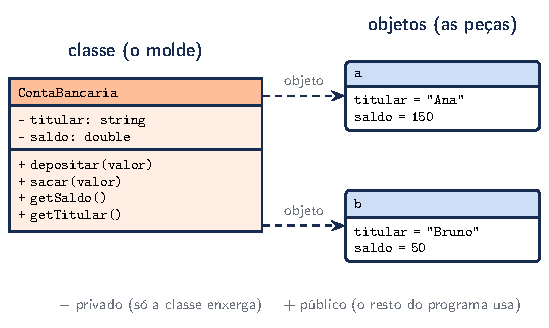
\includegraphics[width=0.85\linewidth,keepaspectratio]{imagens/capitulo-12_classe.pdf}
\end{center}

Em C++, uma classe é declarada com \texttt{class}, de forma parecida com o \texttt{struct}, mas com os métodos dentro dela:

\begin{codigo}
\begin{Verbatim}[breaklines=true, breaksymbolleft={}, fontsize=\footnotesize]
#include <iostream>
#include <string>
using namespace std;

class ContaBancaria {
private:                      // só a própria classe enxerga
    string titular;
    double saldo;

public:                       // o que o resto pode usar
    ContaBancaria(const string &nome, double inicial)
        : titular(nome), saldo(inicial >= 0 ? inicial : 0) {}

    bool depositar(double valor) {
        if (valor <= 0) return false;
        saldo += valor;
        return true;
    }

    bool sacar(double valor) {
        if (valor <= 0 || valor > saldo) return false;
        saldo -= valor;
        return true;
    }

    double getSaldo() const { return saldo; }
    string getTitular() const { return titular; }
};

int main() {
    ContaBancaria a("Ana", 100);          // dois objetos
    ContaBancaria b("Bruno", 50);
    a.depositar(50);
    if (!b.sacar(80)) cout << "Saque recusado" << endl;
    cout << a.getTitular() << ": " << a.getSaldo() << endl;
    cout << b.getTitular() << ": " << b.getSaldo() << endl;
    // b.saldo = 1000000;    erro: saldo é privado
    return 0;
}
// Saque recusado    Ana: 150    Bruno: 50
\end{Verbatim}
\end{codigo}

Um método é chamado com o ponto, como um campo de registro: \texttt{a.depositar(50)} pede ao objeto \texttt{a} que deposite 50 \textbf{na sua própria conta}. Dentro do método, \texttt{saldo} é o saldo do objeto que recebeu a chamada; por isso o mesmo método serve para a conta da Ana e para a do Bruno. O \texttt{const} depois de \texttt{getSaldo()} promete que o método só consulta o objeto, sem alterá-lo.

\subsection{12.2 Construtores e encapsulamento}

O método com o mesmo nome da classe, e sem tipo de retorno, é o \textbf{construtor}: ele é executado automaticamente quando o objeto é criado, e garante que todo objeto já nasce em um estado válido. A linha \texttt{: titular(nome), saldo(...)}, chamada de \textbf{lista de inicialização}, dá os valores iniciais aos atributos; aqui, um saldo inicial negativo vira 0.

As palavras \texttt{private} e \texttt{public} controlam o acesso. Os atributos são \textbf{privados}: só os métodos da própria classe podem lê-los ou alterá-los, e a linha \texttt{b.saldo = 1000000} nem compila. O resto do programa só mexe no saldo por meio dos métodos \textbf{públicos}, e esses métodos garantem as regras do negócio: não se deposita valor negativo, e não se saca mais do que o saldo. Esse princípio, esconder os dados e expor só as operações, é o \textbf{encapsulamento}. Ele tem dois ganhos:

\begin{itemize}
  \item \textbf{Segurança}: as regras ficam em um único lugar, e nenhuma parte do programa consegue deixar uma conta com saldo inválido, nem por engano.
  \item \textbf{Liberdade para mudar}: como ninguém depende de como os dados são guardados por dentro, a implementação pode mudar (guardar o saldo em centavos, registrar um histórico) sem quebrar o resto do programa.
\end{itemize}

Os métodos que só devolvem um atributo, como \texttt{getSaldo}, são chamados de \textbf{getters}. Note que não há um \texttt{setSaldo}: o saldo só muda por depósitos e saques, e é justamente isso que a classe quer garantir.

\subsection{12.3 Herança e polimorfismo}

Muitas vezes, várias classes compartilham uma ideia comum. Um retângulo e um círculo são \textbf{formas}: os dois têm área, mas cada um a calcula de um jeito. A \textbf{herança} permite declarar uma classe \texttt{Forma} com o que é comum, e classes \texttt{Retangulo} e \texttt{Circulo} que \textbf{herdam} dela e completam o que é específico. A relação é de ``é um'': todo retângulo \textbf{é uma} forma.

\begin{center}
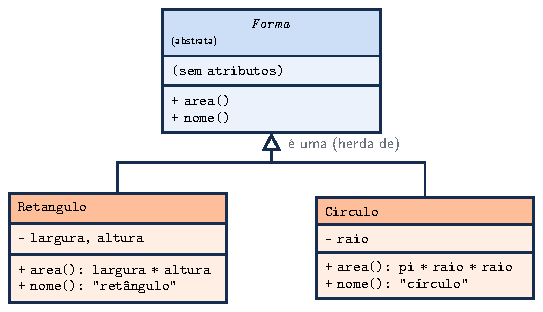
\includegraphics[width=0.75\linewidth,keepaspectratio]{imagens/capitulo-12_heranca.pdf}
\end{center}

\begin{codigo}
\begin{Verbatim}[breaklines=true, breaksymbolleft={}, fontsize=\footnotesize]
#include <iostream>
#include <string>
using namespace std;

class Forma {
public:
    virtual double area() const = 0;      // cada forma calcula
    virtual string nome() const = 0;      // a sua
    virtual ~Forma() {}
};

class Retangulo : public Forma {          // Retangulo é uma Forma
private:
    double largura, altura;
public:
    Retangulo(double l, double a) : largura(l), altura(a) {}
    double area() const override { return largura * altura; }
    string nome() const override { return "retângulo"; }
};

class Circulo : public Forma {
private:
    double raio;
public:
    Circulo(double r) : raio(r) {}
    double area() const override {
        return 3.14159265 * raio * raio;
    }
    string nome() const override { return "círculo"; }
};

void mostrar(const Forma &f) {            // aceita qualquer forma
    cout << f.nome() << ": área " << f.area() << endl;
}

int main() {
    Retangulo r(3, 4);
    Circulo c(1);
    mostrar(r);                           // retângulo: área 12
    mostrar(c);                           // círculo: área 3.14159
    return 0;
}
\end{Verbatim}
\end{codigo}

A classe \texttt{Forma} declara os métodos \texttt{area} e \texttt{nome} como \texttt{virtual ... = 0}: ela diz que toda forma \textbf{tem} esses métodos, mas não os implementa. Por isso é uma \textbf{classe abstrata}, e não se pode criar um objeto \texttt{Forma} sozinho. Cada classe filha implementa os métodos com \texttt{override}, que pede ao compilador para conferir que eles realmente substituem os da classe mãe. O destrutor virtual (\texttt{\textasciitilde Forma}) é uma exigência técnica do C++ para classes que serão herdadas.

O ponto alto está na função \texttt{mostrar}. Ela recebe uma \texttt{Forma} qualquer e chama \texttt{f.area()} sem saber se é um retângulo ou um círculo, e mesmo assim o cálculo certo é executado. Esse comportamento, uma mesma chamada que se adapta ao tipo real do objeto, é o \textbf{polimorfismo}. Ele permite acrescentar um triângulo ao programa sem mudar nenhuma linha de \texttt{mostrar}.

Classes, objetos, encapsulamento, herança e polimorfismo são os pilares da orientação a objetos. Eles aparecem, com sintaxes diferentes, em todas as linguagens orientadas a objetos. A partir daqui, vamos vê-los em Java.

\subsection{12.4 Conhecendo o Java}

O \textbf{Java} foi lançado em 1995 e está até hoje entre as linguagens mais usadas no mundo, em sistemas de bancos e empresas, servidores web e aplicativos Android. Ele foi projetado desde o início para a orientação a objetos: todo código Java fica dentro de alguma classe.

A principal diferença em relação ao C++ está na forma de execução. O compilador do C++ gera código de máquina para um processador e um sistema operacional específicos: um \texttt{.exe} do Windows não roda no Linux. O compilador do Java, o \texttt{javac}, gera um código intermediário, o \textbf{bytecode}, guardado em arquivos \texttt{.class}. Quem executa o bytecode é a \textbf{máquina virtual Java} (JVM), um programa que existe para cada sistema operacional. Assim, o mesmo \texttt{.class} roda em qualquer computador que tenha uma JVM, ideia resumida no lema ``escreva uma vez, rode em qualquer lugar''.

\begin{center}
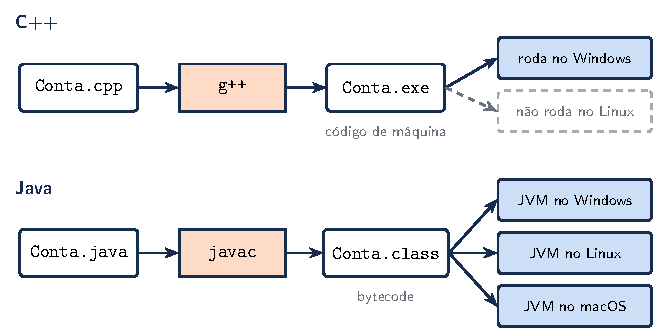
\includegraphics[width=0.9\linewidth,keepaspectratio]{imagens/capitulo-12_jvm.pdf}
\end{center}

O Java também cuida da memória sozinho: não há \texttt{delete}. Um componente da JVM, o \textbf{coletor de lixo} (\textit{garbage collector}), descobre os objetos que nenhuma parte do programa usa mais e devolve a memória deles. Isso elimina os vazamentos e os ponteiros inválidos do Capítulo 11, ao custo de um pouco de controle sobre quando a memória é liberada.

\subsection{12.5 Preparando o ambiente Java}

Para programar em Java é preciso o \textbf{JDK} (\textit{Java Development Kit}), que traz o compilador \texttt{javac}, a máquina virtual e a biblioteca padrão. Os passos são:

\begin{enumerate}
  \item \textbf{Baixe o JDK.} Há distribuições gratuitas, como o Eclipse Temurin (do projeto Adoptium) e o Oracle JDK. Escolha a versão marcada como \textbf{LTS} (\textit{long-term support}, suporte de longo prazo) mais recente, como o JDK 25, e o instalador do seu sistema operacional.
  \item \textbf{Instale.} No Windows, durante a instalação, marque as opções que configuram o \texttt{PATH} e a variável \texttt{JAVA\_HOME}, para que os comandos funcionem em qualquer pasta.
  \item \textbf{Confira.} Abra um terminal novo e digite \texttt{java -version} e \texttt{javac -version}. Os dois devem mostrar a versão instalada. Se aparecer ``comando não encontrado'', o \texttt{PATH} não foi configurado.
  \item \textbf{Escolha uma IDE.} Um ambiente de desenvolvimento integrado reúne editor, compilação, execução e depurador. As mais usadas para Java são o IntelliJ IDEA (que tem uma versão gratuita), o Eclipse, o Apache NetBeans e o Visual Studio Code com as extensões de Java. Ao criar um projeto, a IDE pede para escolher o JDK: aponte para o que você instalou.
\end{enumerate}

Para o primeiro programa, crie um arquivo chamado \texttt{Ola.java}. Em Java, uma classe pública precisa ficar em um arquivo com \textbf{exatamente} o mesmo nome dela, incluindo as maiúsculas:

\begin{codigo}
\begin{Verbatim}[breaklines=true, breaksymbolleft={}, fontsize=\footnotesize]
public class Ola {
    public static void main(String[] args) {
        System.out.println("Olá, Java!");
    }
}
\end{Verbatim}
\end{codigo}

Na IDE, basta clicar em executar. No terminal, compila-se com \texttt{javac}, que gera o \texttt{Ola.class}, e executa-se com \texttt{java}, informando o nome da classe (sem extensão):

\begin{codigo}
\begin{Verbatim}[breaklines=true, breaksymbolleft={}, fontsize=\footnotesize]
$ javac Ola.java
$ java Ola
Olá, Java!
\end{Verbatim}
\end{codigo}

O \texttt{main} do Java tem sempre esse cabeçalho: \texttt{public} (pode ser chamado de fora), \texttt{static} (pertence à classe, e não a um objeto, porque ainda não há objetos quando o programa começa), \texttt{void} (não devolve nada) e o parâmetro \texttt{String[] args}, um vetor com os argumentos digitados no terminal. O \texttt{System.out.println} mostra um texto e pula a linha; o \texttt{System.out.print}, sem o \texttt{ln}, não pula.

\subsection{12.6 Do C++ para o Java}

Quem já programa em C++ reconhece quase toda a sintaxe do Java: tipos, operadores, \texttt{if}, \texttt{switch}, \texttt{while}, \texttt{for} e funções são praticamente iguais. As diferenças principais estão na tabela:

\begin{center}
\begin{tabular}{@{}p{0.2\linewidth}p{0.33\linewidth}p{0.35\linewidth}@{}}
\toprule
\rowcolor{headergray}
\tblheader{Recurso} & \tblheader{C++} & \tblheader{Java} \\
\midrule
saída & \texttt{cout << x << endl;} & \texttt{System.out.println(x);} \\
\rowcolor{rowgray} entrada & \texttt{cin >> x;} & \texttt{x = entrada.nextInt();} (com \texttt{Scanner}) \\
lógico & \texttt{bool} & \texttt{boolean} \\
\rowcolor{rowgray} texto & \texttt{string} & \texttt{String} \\
vetor & \texttt{int v[5];} & \texttt{int[] v = new int[5];} \\
\rowcolor{rowgray} tamanho variável & \texttt{vector<int>} & \texttt{ArrayList<Integer>} \\
funções & podem ficar fora de classes & sempre dentro de uma classe (métodos) \\
\rowcolor{rowgray} memória & \texttt{new} e \texttt{delete} & \texttt{new}; o coletor de lixo libera \\
comparar textos & \texttt{a == b} & \texttt{a.equals(b)} \\
\bottomrule
\end{tabular}
\end{center}

Os vetores do Java sabem o próprio tamanho (\texttt{v.length}) e, ao contrário do C++, \textbf{conferem os índices}: acessar \texttt{v[5]} em um vetor de 5 elementos interrompe o programa com uma \texttt{ArrayIndexOutOfBoundsException}, em vez do comportamento indefinido do Capítulo 7. O programa abaixo lê notas com a classe \texttt{Scanner}, até o usuário digitar um valor negativo, e mostra a média:

\begin{codigo}
\begin{Verbatim}[breaklines=true, breaksymbolleft={}, fontsize=\footnotesize]
import java.util.ArrayList;
import java.util.Locale;
import java.util.Scanner;

public class MediaNotas {
    public static void main(String[] args) {
        Scanner entrada = new Scanner(System.in);
        entrada.useLocale(Locale.US);      // 7.5 com ponto
        ArrayList<Double> notas = new ArrayList<>();
        System.out.print("Notas (negativo para terminar): ");
        while (entrada.hasNextDouble()) {
            double nota = entrada.nextDouble();
            if (nota < 0) break;
            notas.add(nota);
        }
        double soma = 0;
        for (double nota : notas) soma += nota;
        if (!notas.isEmpty()) {
            System.out.println(notas.size() + " notas, média "
                               + soma / notas.size());
        }
    }
}
// Entrada: 7 4.5 9 6 -1  ->  4 notas, média 6.625
\end{Verbatim}
\end{codigo}

O \texttt{Scanner} lê números conforme as convenções do idioma do computador. Em um computador configurado em português, ele espera a vírgula decimal (\texttt{7,5}) e recusa \texttt{7.5}. A linha com \texttt{Locale.US} fixa o ponto decimal, para que o programa se comporte igual em qualquer máquina. O \texttt{+} entre um texto e um número junta os dois em um texto, como na concatenação de strings do C++.

\subsection{12.7 Classes em Java}

A conta bancária em Java fica muito parecida com a versão em C++. As diferenças: cada atributo e método recebe seu próprio \texttt{private} ou \texttt{public}, o construtor não tem lista de inicialização, e os objetos são sempre criados com \texttt{new}.

\begin{codigo}
\begin{Verbatim}[breaklines=true, breaksymbolleft={}, fontsize=\footnotesize]
public class ContaBancaria {
    private String titular;
    private double saldo;

    public ContaBancaria(String titular, double inicial) {
        this.titular = titular;      // this: o atributo do objeto
        this.saldo = inicial >= 0 ? inicial : 0;
    }

    public boolean depositar(double valor) {
        if (valor <= 0) return false;
        saldo += valor;
        return true;
    }

    public boolean sacar(double valor) {
        if (valor <= 0 || valor > saldo) return false;
        saldo -= valor;
        return true;
    }

    public double getSaldo() { return saldo; }
    public String getTitular() { return titular; }

    public static void main(String[] args) {
        ContaBancaria a = new ContaBancaria("Ana", 100);
        ContaBancaria b = new ContaBancaria("Bruno", 50);
        a.depositar(50);
        if (!b.sacar(80)) System.out.println("Saque recusado");
        System.out.println(a.getTitular() + ": " + a.getSaldo());
        System.out.println(b.getTitular() + ": " + b.getSaldo());
    }
}
// Saque recusado    Ana: 150.0    Bruno: 50.0
\end{Verbatim}
\end{codigo}

No construtor, o parâmetro \texttt{titular} tem o mesmo nome do atributo. A palavra \texttt{this}, que significa ``este objeto'', desfaz a ambiguidade: \texttt{this.titular} é o atributo, e \texttt{titular} sozinho é o parâmetro. Repare também que o Java mostra \texttt{150.0}: um \texttt{double} sempre é exibido com a parte decimal.

Em Java, uma variável de objeto, como \texttt{a}, guarda uma \textbf{referência} para o objeto, parecida com um ponteiro, mas sem aritmética nem \texttt{delete}. Por isso, \texttt{ContaBancaria c = a;} não copia a conta: \texttt{c} e \texttt{a} passam a ser dois nomes para o \textbf{mesmo} objeto, e um depósito feito por \texttt{c} aparece no saldo de \texttt{a}. Uma referência que não aponta para nenhum objeto vale \texttt{null}, o equivalente ao \texttt{nullptr}.

\subsection{12.8 Herança em Java}

A herança em Java usa a palavra \texttt{extends}, e a anotação \texttt{@Override} faz o papel do \texttt{override} do C++. Em Java, todos os métodos são polimórficos por padrão, sem precisar de \texttt{virtual}. Uma classe abstrata é marcada com \texttt{abstract}:

\begin{codigo}
\begin{Verbatim}[breaklines=true, breaksymbolleft={}, fontsize=\footnotesize]
import java.util.ArrayList;

abstract class Forma {
    public abstract double area();
    public abstract String nome();
}

class Retangulo extends Forma {
    private double largura, altura;

    public Retangulo(double largura, double altura) {
        this.largura = largura;
        this.altura = altura;
    }
    @Override public double area() { return largura * altura; }
    @Override public String nome() { return "retângulo"; }
}

class Circulo extends Forma {
    private double raio;

    public Circulo(double raio) { this.raio = raio; }
    @Override public double area() {
        return Math.PI * raio * raio;
    }
    @Override public String nome() { return "círculo"; }
}

public class Formas {
    public static void main(String[] args) {
        ArrayList<Forma> formas = new ArrayList<>();
        formas.add(new Retangulo(3, 4));
        formas.add(new Circulo(1));
        formas.add(new Retangulo(2, 2.5));
        for (Forma f : formas) {               // polimorfismo
            System.out.println(f.nome() + ": área " + f.area());
        }
    }
}
// retângulo: área 12.0
// círculo: área 3.141592653589793
// retângulo: área 5.0
\end{Verbatim}
\end{codigo}

A lista \texttt{formas} guarda objetos de classes diferentes, todos tratados como \texttt{Forma}, e o laço chama o \texttt{area()} de cada um sem saber qual é a classe real. Um arquivo pode ter várias classes, mas só uma pública, que dá nome ao arquivo: aqui, \texttt{Formas.java}.

\subsection{12.9 Um programa completo: uma pequena biblioteca}

O programa abaixo reúne os conceitos do capítulo em um sistema de empréstimo de livros. A classe \texttt{Livro} encapsula os dados de um livro e a regra de que um livro emprestado não pode ser emprestado de novo. A classe \texttt{Biblioteca} guarda o acervo em um \texttt{ArrayList} e oferece cadastro, busca e listagem. O \texttt{main} só conversa com os objetos, por meio dos seus métodos públicos.

\begin{codigo}
\begin{Verbatim}[breaklines=true, breaksymbolleft={}, fontsize=\footnotesize]
import java.util.ArrayList;

class Livro {
    private String titulo;
    private String autor;
    private boolean emprestado = false;   // nasce disponível

    public Livro(String titulo, String autor) {
        this.titulo = titulo;
        this.autor = autor;
    }

    public String getTitulo() { return titulo; }
    public boolean isEmprestado() { return emprestado; }

    public boolean emprestar() {
        if (emprestado) return false;     // já está com alguém
        emprestado = true;
        return true;
    }

    public void devolver() { emprestado = false; }

    @Override
    public String toString() {            // o livro como texto
        return titulo + " (" + autor + ")"
               + (emprestado ? " - emprestado" : "");
    }
}

class Biblioteca {
    private ArrayList<Livro> acervo = new ArrayList<>();

    public void cadastrar(Livro livro) { acervo.add(livro); }

    public Livro buscar(String titulo) {
        for (Livro l : acervo) {
            if (l.getTitulo().equalsIgnoreCase(titulo)) return l;
        }
        return null;                      // não encontrado
    }

    public int disponiveis() {
        int total = 0;
        for (Livro l : acervo) {
            if (!l.isEmprestado()) total++;
        }
        return total;
    }

    public void listar() {
        for (Livro l : acervo) System.out.println("  " + l);
    }
}

public class SistemaBiblioteca {
    public static void main(String[] args) {
        Biblioteca bib = new Biblioteca();
        bib.cadastrar(new Livro("Dom Casmurro",
                                "Machado de Assis"));
        bib.cadastrar(new Livro("Vidas Secas",
                                "Graciliano Ramos"));
        bib.cadastrar(new Livro("O Cortiço", "Aluísio Azevedo"));

        Livro livro = bib.buscar("vidas secas");  // minúsculas
        if (livro != null) {
            System.out.println("1o pedido: " + livro.emprestar());
            System.out.println("2o pedido: " + livro.emprestar());
        }
        bib.listar();
        System.out.println(bib.disponiveis() + " disponíveis");
        if (bib.buscar("Iracema") == null) {
            System.out.println("Iracema não está no acervo");
        }
    }
}
\end{Verbatim}
\end{codigo}

A saída mostra a regra do empréstimo funcionando: o primeiro pedido é aceito e o segundo, recusado, porque o livro já está emprestado.

\begin{codigo}
\begin{Verbatim}[breaklines=true, breaksymbolleft={}, fontsize=\footnotesize]
// saída
1o pedido: true
2o pedido: false
  Dom Casmurro (Machado de Assis)
  Vidas Secas (Graciliano Ramos) - emprestado
  O Cortiço (Aluísio Azevedo)
2 disponíveis
Iracema não está no acervo
\end{Verbatim}
\end{codigo}

Três detalhes de Java aparecem aqui. O método \texttt{toString}, que toda classe herda de uma classe-mãe comum chamada \texttt{Object}, define como o objeto vira texto; por isso \texttt{"  " + l} mostra o livro formatado. A busca compara títulos com \texttt{equalsIgnoreCase}, que ignora maiúsculas e minúsculas. E \texttt{buscar} devolve \texttt{null} quando não acha, o que obriga quem chama a testar antes de usar o resultado, como no \texttt{if (livro != null)}.

Para continuar, experimente acrescentar ao sistema uma classe \texttt{Usuario}, um limite de livros por usuário, ou uma busca por autor. Cada nova regra deve ficar dentro da classe a que ela pertence: esse é o hábito central da orientação a objetos.

\subsection{Erros Comuns}

\begin{itemize}
  \item \textbf{Deixar os atributos públicos.} Qualquer parte do programa passa a poder quebrar as regras da classe. Atributos privados, métodos públicos.
  \item \textbf{Esquecer o ponto e vírgula depois da classe em C++.} Como no \texttt{struct}, a declaração termina com \texttt{\};}. Em Java, não há ponto e vírgula depois da classe.
  \item \textbf{Esquecer o \texttt{virtual} em C++.} Sem ele, \texttt{mostrar(r)} chama o método de \texttt{Forma}, e não o do retângulo.
  \item \textbf{Nome do arquivo diferente do nome da classe pública em Java.} A classe \texttt{Ola} precisa estar em \texttt{Ola.java}, com as mesmas maiúsculas.
  \item \textbf{Comparar textos com \texttt{==} em Java.} O \texttt{==} compara se são o mesmo objeto, e não se têm o mesmo conteúdo. Use \texttt{a.equals(b)}.
  \item \textbf{Usar uma referência \texttt{null}.} Chamar um método em \texttt{null} interrompe o programa com uma \texttt{NullPointerException}. Teste antes, como em \texttt{if (livro != null)}.
  \item \textbf{Achar que \texttt{b = a} copia o objeto em Java.} As duas variáveis passam a apontar para o mesmo objeto.
  \item \textbf{Esquecer o \texttt{new} em Java.} Declarar \texttt{ContaBancaria c;} não cria nenhuma conta; só \texttt{new ContaBancaria(...)} cria.
\end{itemize}
